\chapter{Analyse}

I dette kapitel vil vi gennemgå kravspecifikation til programmet, samt optegne og forklare forskellige modeller.


\section{Kravspecifikation}

\begin{enumerate}
    \item Spillet skal håndtere to spillere.
    \item Man skal slå med to terninger, som begge er fair.
    \item Summen af de to terningerner ligges sammen og gives til spillerens pointsum.
    \item Man vinder ved at nå 40 point.
    \item Ved at slå to 1'ere, nulstilles spillerens point.
    \item To ens giver ekstra tur.
    \item Skal kunne huske spillerens forrige kast.
    \item Spilleren kan vinde med at slå to 6'ere i forrige kast og nuværende kast.
    \item To ens for at vinde spillet efter 40 point.
\end{enumerate}

\section{Interessentanalyse}

\begin{center}
    \begin{tabular}{ | l | p{13cm} |}
    \hline
    \textbf{Interresent} & \textbf{Interesse / Mål} \\ \hline
    Spiller/-e & Kunne styre et system, der styrer et spil mellem 2 personer, 
    hvor i der kastes med et raflebæger med to terninger i og ser resultatet med det samme. \\ \hline
    \hline
    \end{tabular}
\end{center}

\section{Use cases}

\begin{table}[H]
    \begin{center}
        \begin{tabular}{ | p{15cm} |}
            \hline
            \textbf{Use case:} PlayGame \\ \hline
            \textbf{ID:} 1 \\ \hline
            \textbf{Brief description} Spiller/-e skal kunne spille spil/Game (starte spillet) og slå med terningen     \\ \hline
            \textbf{Primary actors:} Spiller/-e \\ \hline
            \textbf{Secondary actors:} Ingen. \\ \hline
            \textbf{Preconditions:} Ingen.     \\ \hline
            \textbf{Main flow:}
            \begin{enumerate}
                \item \textbf{Spiller 1 indtaster navn}
                \item \textbf{Spiller 2 indtaster navn}
                \item \textbf{Spiller 1 indtaster 'roll' for at slå med terningen}
                \item \textbf{Spiller 2 indtaster 'roll' for at slå med terningen}
                \item \textbf{Opnås 40 point, og to ens terninger slås, stoppes spillet}    
            \end{enumerate} \\ \hline
            \textbf{Postconditions:} Ingen.\\ \hline
            \textbf{Alternative flow:}
            \\- Ekstra ture gives ved, at slå to ens terninger
            \\- Slås to ens, med 1’ere bliver spillerens score nulstillet
            \\- Spil afsluttes, hvis der bliver slået to 6’ere, med den forudsætning, at to 6’ere blev slået i den forrige runde  \\ \hline
            \hline
        \end{tabular}
        \caption{Use case 1}
        \label{usecase:1}
    \end{center}
\end{table}

\newpage

\section{Domænemodel}

For bedre at kunne forstå domænet omkring spillet, har vi ud fra use case 1 (Tabel \ref{usecase:1}) lavet en domænemodel. domænemodellen beskriver de elementer vi vil arbejde med.
Det ses der, at spillet kommer til at bestå af terningerne og spillere.
På figur \ref{fig:domaenemodel} ses domænet.
Der ses at både terninger (Dice) og spillere (Player) refererer til spillet (Game).

\begin{figure}[h]
    \begin{center}
        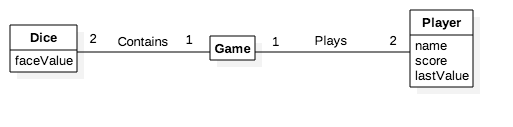
\includegraphics[width=15cm]{graphics/Domaenemodel}
        \caption{Domænemodel over spillet}
        \label{fig:domaenemodel}
    \end{center}
\end{figure}